\documentclass[a4paper]{article}

% bloc : évite un changement de page
% completemulti : ajoute une case : aucune bonne réponse
%\newcommand{\repRel}{../..}
%\input{\repRel/Style/packages}
%%\input{\repRel/Style/new_style}
%\input{\repRel/Style/macros_SII}
%%\input{\repRel/Style/environment}

%\usepackage[francais,bloc,completemulti,ensemble]{automultiplechoice}
\usepackage[francais,bloc,completemulti,catalog]{automultiplechoice} %ensemble
\usepackage{multicol}

%% Pour le python %%
\usepackage{listingsutf8}
\usepackage{amsmath}

\lstset{language=Python,
  inputencoding=utf8/latin1,
  breaklines=true,
  basicstyle=\ttfamily\small,
  keywordstyle=\bfseries\color{green!40!black},
  commentstyle=\itshape\color{purple!40!black},
  identifierstyle=\color{blue},
  stringstyle=\color{orange},
  upquote = true,
  columns=fullflexible,
  backgroundcolor=\color{gray!10},frame=leftline,rulecolor=\color{gray}}  
  
\definecolor{mygreen}{rgb}{0,0.6,0}

\lstset{
     literate=%
         {é}{{\'e}}1    
         {è}{{\`e}}1    
         {ê}{{\^e}}1    
         {à}{{\`a}}1
         {â}{{\^a}}1		 
         {ô}{{\^o}}1    
         {ù}{{\`u}}1    
         {î}{{\^i}}1    
}
\lstset{inputpath=../Banque_Info/code}

%\usepackage[utf8x]{inputenc}
%\usepackage[T1]{fontenc}

\begin{document}
\graphicspath{{../Banque_SI/05_inertieeq/images}}
\element{inertieeq}{
\begin{question}{jeq 01}
Soit le schéma suivant. Déterminer l'inertie équivalente ramenée à l'arbre moteur 1.
\begin{center}
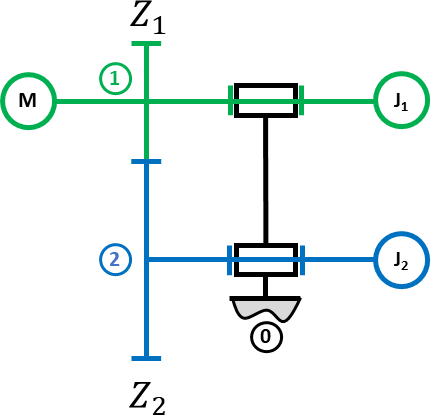
\includegraphics[width=5cm]{fig_01}
\end{center}
\begin{multicols}{2}
	\begin{reponses}
	% 1/2 J_1 \omega_1^2 + 1/2 J_2 \omega_1^2 Z_1^2/Z_2^2 
	\bonne     {$J_1                                  +  \dfrac{Z_1^2}{Z_2^2} J_2$}
	\mauvaise{$\dfrac{Z_2^2}{Z_1^2}J_1 + J_2$}
	\mauvaise{$J_1                                  +  \dfrac{Z_2^2}{Z_1^2} J_2$}
	\mauvaise{$\dfrac{Z_1^2}{Z_2^2}J_1 + J_2  $}
	\end{reponses}
\end{multicols}
\end{question}\\}


\element{inertieeq}{
\begin{question}{jeq 02}
Soit le schéma suivant. Déterminer l'inertie équivalente ramenée à l'arbre 2.
\begin{center}
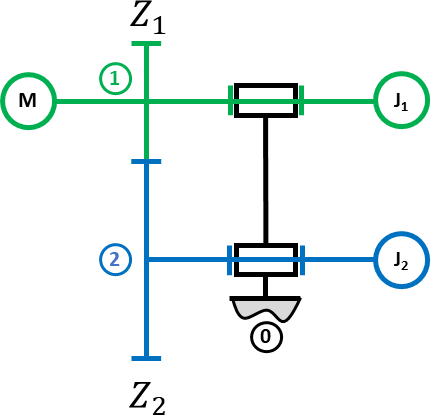
\includegraphics[width=5cm]{fig_01}
\end{center}
\begin{multicols}{2}
	\begin{reponses}
	% 1/2 J_1 \omega_1^2 + 1/2 J_2 \omega_1^2 Z_1^2/Z_2^2 
	\bonne {$\dfrac{Z_2^2}{Z_1^2}J_1 + J_2    $}
	\mauvaise{$J_1 + \dfrac{Z_1^2}{Z_2^2} J_2$}
	\mauvaise{$J_1 + \dfrac{Z_2^2}{Z_1^2}J_2 $}
	\mauvaise{$\dfrac{Z_1^2}{Z_2^2}J_1 + J_2 $}
	\end{reponses}
\end{multicols}
\end{question}\\}


%%%%%%%%%%%%%%%
\element{inertieeq}{
\begin{question}{jeq 03}
Soit le schéma suivant. Déterminer l'inertie équivalente ramenée à l'arbre moteur 1.
\begin{center}
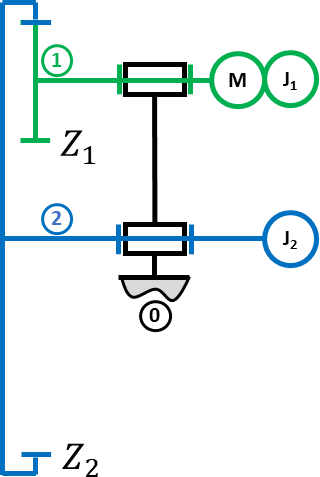
\includegraphics[width=5cm]{fig_02}
\end{center}
\begin{multicols}{2}
	\begin{reponses}
	\bonne     {$ J_1 +  \dfrac{Z_1^2}{Z_2^2} J_2 $}
	\mauvaise{$ \dfrac{Z_2^2}{Z_1^2}J_1 + J_2   $}
	\mauvaise{$ J_1 +  \dfrac{Z_2^2}{Z_1^2} J_2 $}
	\mauvaise{$ \dfrac{Z_1^2}{Z_2^2}J_1 + J_2   $}
	\end{reponses}
\end{multicols}
\end{question}\\}

\element{inertieeq}{
\begin{question}{jeq 04}
Soit le schéma suivant. Déterminer l'inertie équivalente ramenée à l'arbre 2.
\begin{center}
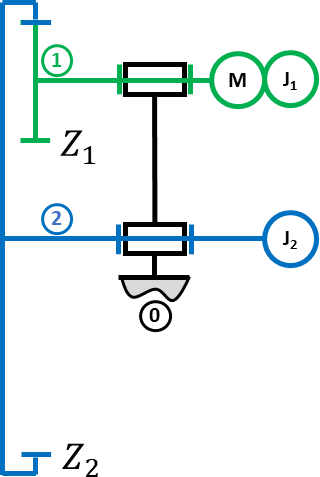
\includegraphics[width=5cm]{fig_02}
\end{center}
\begin{multicols}{2}
	\begin{reponses}
	\bonne     {$ \dfrac{Z_2^2}{Z_1^2}J_1 + J_2 $}
	\mauvaise{$ J_1 + \dfrac{Z_1^2}{Z_2^2} J_2 $}
	\mauvaise{$ J_1 + \dfrac{Z_2^2}{Z_1^2}J_2 $}
	\mauvaise{$ \dfrac{Z_1^2}{Z_2^2}J_1 + J_2 $}
	\end{reponses}
\end{multicols}
\end{question}\\}
%%%%%%%%%%%%

%%%%%%%%%%%%%%%
\element{inertieeq}{
\begin{question}{jeq 05}
Soit le schéma suivant. Déterminer l'inertie équivalente ramenée à l'arbre moteur 1.
\begin{center}
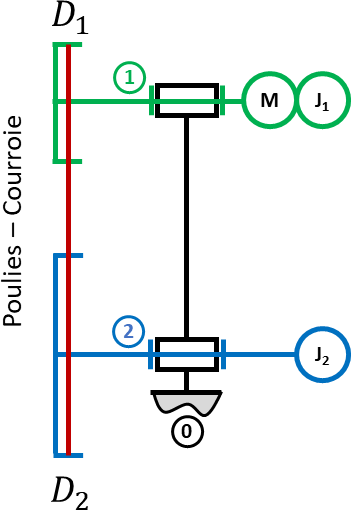
\includegraphics[width=5cm]{fig_03}
\end{center}
\begin{multicols}{2}
	\begin{reponses}
	\bonne     {$ J_1 +  \dfrac{D_1^2}{D_2^2} J_2 $}
	\mauvaise{$  \dfrac{D_2^2}{D_1^2}J_1 + J_2   $}
	\mauvaise{$  J_1 +  \dfrac{D_2^2}{D_1^2} J_2 $}
	\mauvaise{$ \dfrac{D_1^2}{D_2^2}J_1 + J_2   $}
	\end{reponses}
\end{multicols}
\end{question}\\}

\element{inertieeq}{
\begin{question}{jeq 06}
Soit le schéma suivant. Déterminer l'inertie équivalente ramenée à l'arbre 2.
\begin{center}
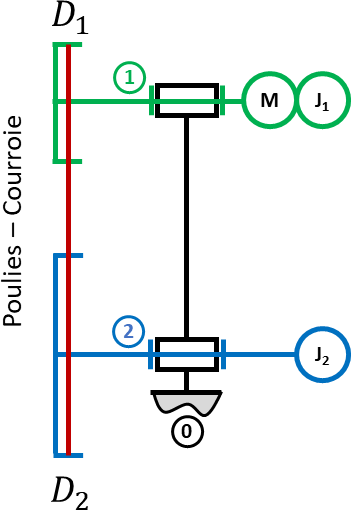
\includegraphics[width=5cm]{fig_03}
\end{center}
\begin{multicols}{2}
	\begin{reponses}
	\bonne     {$ \dfrac{D_2^2}{D_1^2}J_1 + J_2    $}
	\mauvaise{$   J_1 + \dfrac{D_1^2}{D_2^2} J_2  $}
	\mauvaise{$  J_1 + \dfrac{D_2^2}{D_1^2}J_2    $}
	\mauvaise{$  \dfrac{D_1^2}{D_2^2}J_1 + J_2    $}
	\end{reponses}
\end{multicols}
\end{question}\\}
%%%%%%%%%%%%


%%%%%%%%%%%%%%%
\element{inertieeq}{
\begin{question}{jeq 07}
Soit le schéma suivant. Déterminer l'inertie équivalente ramenée à l'arbre moteur 1.
\begin{center}
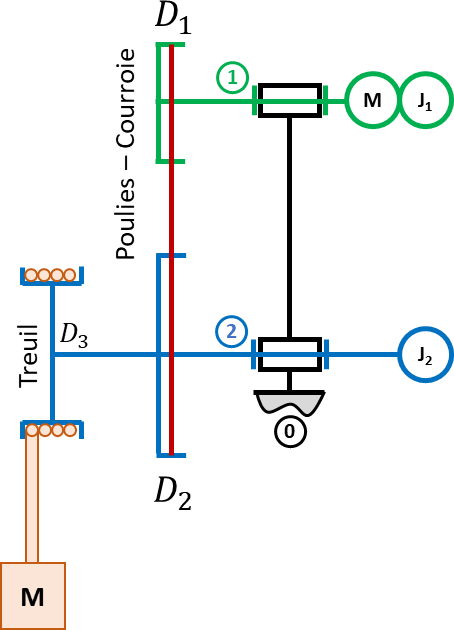
\includegraphics[width=5cm]{fig_04}
\end{center}
% omega_2 = omega_1 \dfrac{D_1}{D_2} 
% v = D3/2 omega_2
% 1/2 (J_1 omega_1^2 + J_2 omega_2^2 + Mv^2)
% 1/2 omega_1^2 (J_1  + J_2  \dfrac{D_1}{D_2}^2 + M (D3/2)^2\dfrac{D_1}{D_2}^2 )

\begin{multicols}{2}
	\begin{reponses}
	\bonne      {$J_1  + J_2  \left(\dfrac{D_1}{D_2}\right)^2 + M \left(\dfrac{D_1D_3}{2D_2}\right)^2$}
	\mauvaise {$J_1 \left(\dfrac{D_2}{D_1}\right)^2 + J_2  + M\left(\dfrac{D_3}{2}\right)^2$}
	\mauvaise {$J_1  + J_2  \left(\dfrac{D_2}{D_1}\right)^2 + M \left(\dfrac{2D_2}{D_1D_3}\right)^2$}
	\mauvaise {$J_1 \left(\dfrac{D_1}{D_2}\right)^2 + J_2  + M \left(\dfrac{D_1D_3}{2D_2}\right)^2$}
	\end{reponses}
\end{multicols}
\end{question}\\}

\element{inertieeq}{
\begin{question}{jeq 08}
Soit le schéma suivant. Déterminer l'inertie équivalente ramenée à l'arbre 2.
\begin{center}
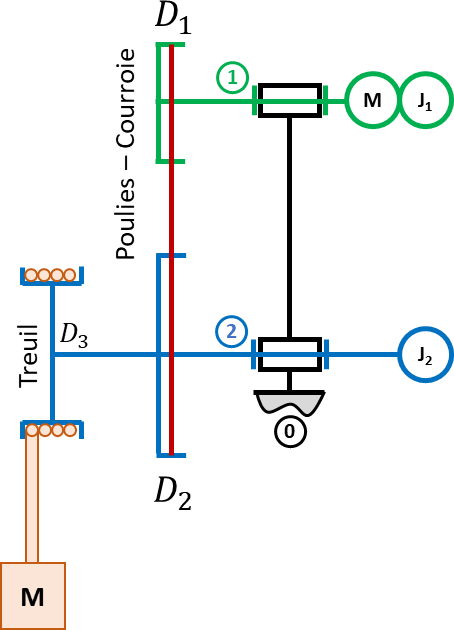
\includegraphics[width=5cm]{fig_04}
\end{center}
% omega_2 = omega_1 \dfrac{D_1}{D_2} 
% v = D3/2 omega_2
% 1/2 (J_1 omega_1^2 + J_2 omega_2^2 + Mv^2)
% 1/2 omega_2^2 (J_1 \left(\dfrac{D_2}{D_1}\right)^2 + J_2  + M\left(\dfrac{D_3}{2}\right)^2)
\begin{multicols}{2}
	\begin{reponses}
	\bonne     {$J_1 \left(\dfrac{D_2}{D_1}\right)^2 + J_2  + M\left(\dfrac{D_3}{2}\right)^2$}
	\mauvaise {$J_1  + J_2  \left(\dfrac{D_1}{D_2}\right)^2 + M \left(\dfrac{D_1D_2}{2D_2}\right)^2$}
	\mauvaise {$J_1  + \left(\dfrac{D_2}{D_1}\right)^2J_2  + M\left(\dfrac{D_3}{2}\right)^2$}
	\mauvaise {$J_1 \left(\dfrac{D_1}{D_2}\right)^2 + J_2  + M\left(\dfrac{D_3}{2}\right)^2$}
	\end{reponses}
\end{multicols}
\end{question}\\}

\element{inertieeq}{
\begin{question}{jeq 09}
Soit le schéma suivant. Déterminer la masse équivalente.
\begin{center}
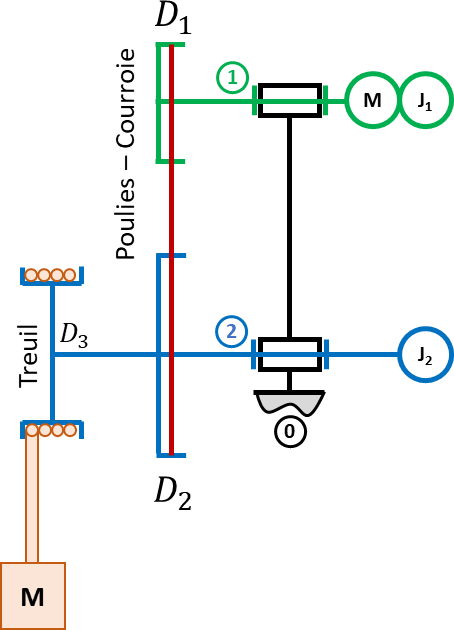
\includegraphics[width=5cm]{fig_04}
\end{center}
% omega_2 = omega_1 \dfrac{D_1}{D_2} 
% v = D3/2 omega_2
% 1/2 (J_1 \dfrac{2D_2}{D_1D_3}^2 + J_2 (2/D3)^2 + Mv^2)
\begin{multicols}{2}
	\begin{reponses}
	\bonne     {$J_1 \left(\dfrac{2D_2}{D_1D_3}\right)^2 + J_2 \left(\dfrac{2}{D3}\right)^2 + M$}
	\mauvaise {$J_1 \left(\dfrac{2}{D3}\right)^2 + J_2 \left(\dfrac{2D_2}{D_1D_3}\right)^2 + M$}
	\mauvaise {$J_1 \left(\dfrac{2D_1}{D_2D_3}\right)^2 + J_2 \left(\dfrac{2}{D3}\right)^2 + M$}
	\mauvaise {$J_1 \left(\dfrac{2D_3}{D_2D_1}\right)^2 + J_2 \left(\dfrac{2}{D3}\right)^2 + M$}
	\end{reponses}
\end{multicols}
\end{question}\\}
%%%%%%%%%%%%






%
%
%
%\element{inertieeq}{
%\begin{question}{jeq 08}
%On note $v$ la vitesse de la charge $M$ selon la direction horizontale. Exprimer $v$ en fonction de
%$\omega_{10}$ (en valeur absolue). On note $m$ le module des roues dentées.
%\begin{center}
%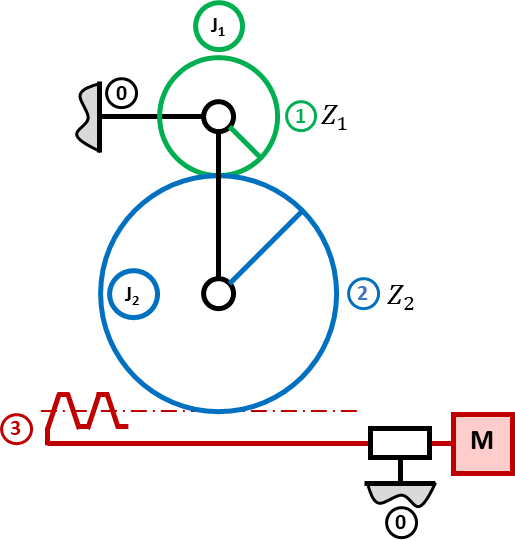
\includegraphics[width=5cm]{fig_05}
%\end{center}
%\begin{multicols}{4}
%	\begin{reponses}	
%	\mauvaise{$v = \dfrac{Z_2}{Z_1 } \omega_{10}$}
%	\mauvaise{$v = \dfrac{m Z_2}{Z_1 } \omega_{10}$}
%	\mauvaise{$v = \dfrac{Z_2^2}{2 Z_1 } \omega_{10}$}
%	\bonne{$v = \dfrac{m Z_2}{2 Z_1 Z_2} \omega_{10}$}
%	\end{reponses}
%\end{multicols}
%\end{question}\\}
%
%\element{inertieeq}{
%\begin{question}{jeq 09}
%Exprimer $\omega_{10}$ en fonction de $\omega_{30}$ (en valeur absolue). 
%\begin{center}
%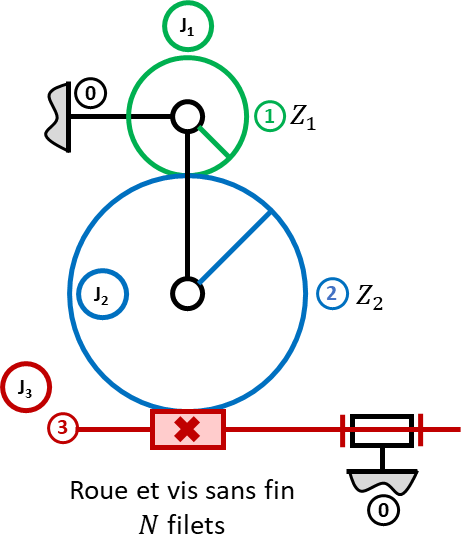
\includegraphics[width=5cm]{fig_06}
%\end{center}
%\begin{multicols}{4}
%	\begin{reponses}	
%	\mauvaise{$\omega_{10} = \dfrac{Z_2^2}{NZ_1}  \omega_{30}$}
%	\mauvaise{$\omega_{10} = \dfrac{N}{Z_2} \dfrac{Z_1}{Z_2} \omega_{30}$}
%	\mauvaise{$\omega_{10} =  NZ_1 \omega_{30}$}
%	\bonne{$\omega_{10} = \dfrac{N}{Z_1} \omega_{30}$}
%	\end{reponses}
%\end{multicols}
%\end{question}\\}
%
%\element{inertieeq}{
%\begin{question}{jeq 10}
%On note $v$ la vitesse de la charge $M$ selon la direction horizontale. Exprimer $v$ en fonction de 
%$\omega_{10}$ (en valeur absolue). On note $p$ le pas de la vis.
%\begin{center}
%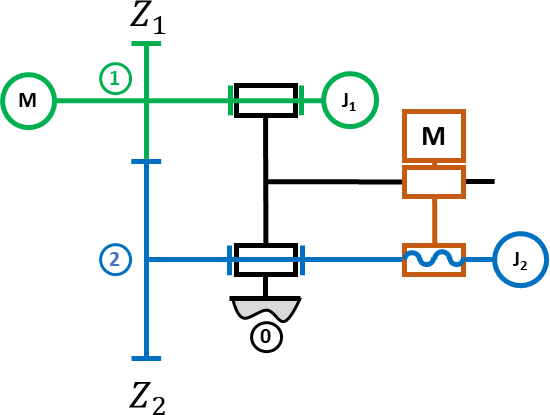
\includegraphics[width=5cm]{fig_07}
%\end{center}
%\begin{multicols}{4}
%	\begin{reponses}	
%	\mauvaise{$v = \dfrac{ Z_2  }{ Z_1  p } \omega_{10}$}
%	\mauvaise{$v = \dfrac{Z_2 p}{2 Z_1  \pi } \omega_{10}$}
%	\mauvaise{$v = \dfrac{2 Z_1 \pi }{ Z_2  p } \omega_{10}$}
%	\bonne{$v = \dfrac{Z_1 p}{2 Z_2  \pi } \omega_{10}$}
%	\end{reponses}
%\end{multicols}
%\end{question}\\}
%






%\melangegroupe{OperationsElementaires}
	%\restituegroupe{transmetteurs}
	\restituegroupe{inertieeq}



	
\end{document}